
\chapter{预等离子体对于加速的增强作用}
\label{chap:preplasmaEhancement}




\section{引言}
\begin{figure}[!htbp]
  \centering
  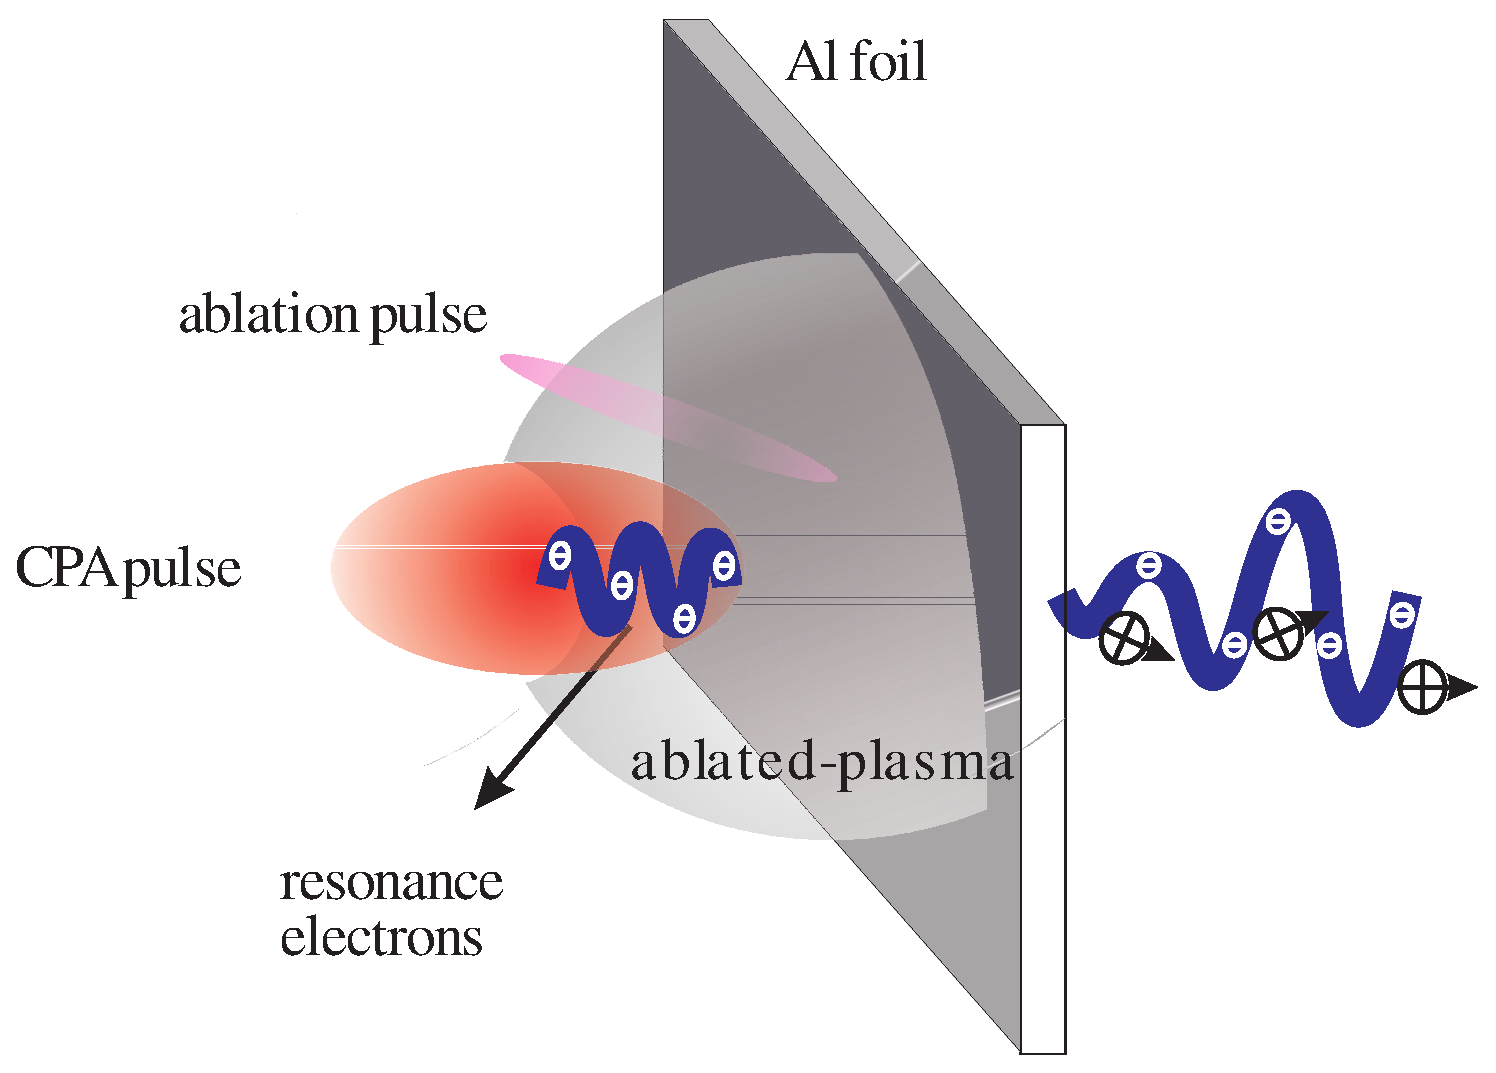
\includegraphics[width=\MyFactor\textwidth]{Img/enhancement.eps}
  \caption{预脉冲增强作用示意图}
  \label{fig:prepulse2012}
\end{figure}

上一章中,我们研究了激光的预脉冲或者中等强度激光脉冲($10^{10}W/cm^2$ 到 $10^{14}W/cm^2$),对于金属靶进行烧蚀过程,以及预等离子体的产生。预等离子体是靶前表面烧蚀的产物,由烧蚀前沿向外传播,同时其压力波向靶内部传播,形成一定的密度压缩。其密度分布较复杂,主要集中在近临界密度区域,且呈现类指数函数分布。我们已经对于临界密度做出定义,当等离子体频率对应于激光频率,此时的等离子体密度为临界密度。有等离子体中的色散关系${\omega}^2={{\omega}_p}^2 +k^2 c^2$知,当等离子体频率高于激光频率时,激光在等离子体中无法传播。因此临界密度也是非相对论激光脉冲穿透的密度极限。然而对于相对论强度激光,由于相对论效应,其色散关系${\omega}^2={{\omega}_p}^2/{\gamma} +k^2 c^2$,其中${{\omega}_p}^2=4 {\pi}^2 n_e/m $,$\gamma$是相对论因子。由于相对论因子的存在,使得激光在高于临界密度的等离子体中传播,这种线性被称为相对论自导引穿透。
在传播过程中,由于激光脉冲强度在横向存在一定分布,一般情况下为高斯分布,因此有质动力在横向上也存在类似的分布,使得横向上电子被排开的程度不同,等离子体的密度分布不再均匀。另一方面,电子的相对论质量也存径向分布,中心处的电子的质量偏大,而两翼出的电子的质量相对较小。其直接效果是,等离子体的折射率的中心处变小,而两边较大。这种由激光脉冲对于等离子体折射率的调制,并改变激光在传播过程中的聚焦属性的现象,称为相对论自聚焦。于此同时,考虑激光的纵向分布,假设纵向分布为高斯分布,激光光强对于包络的群速度产生调制作用,包络峰值处的光强较高群速度较快,使得脉冲峰值处前移,脉冲上升沿变得陡峭,这种现象称为相对论自调制。

\begin{figure}[!htbp]
  \centering
  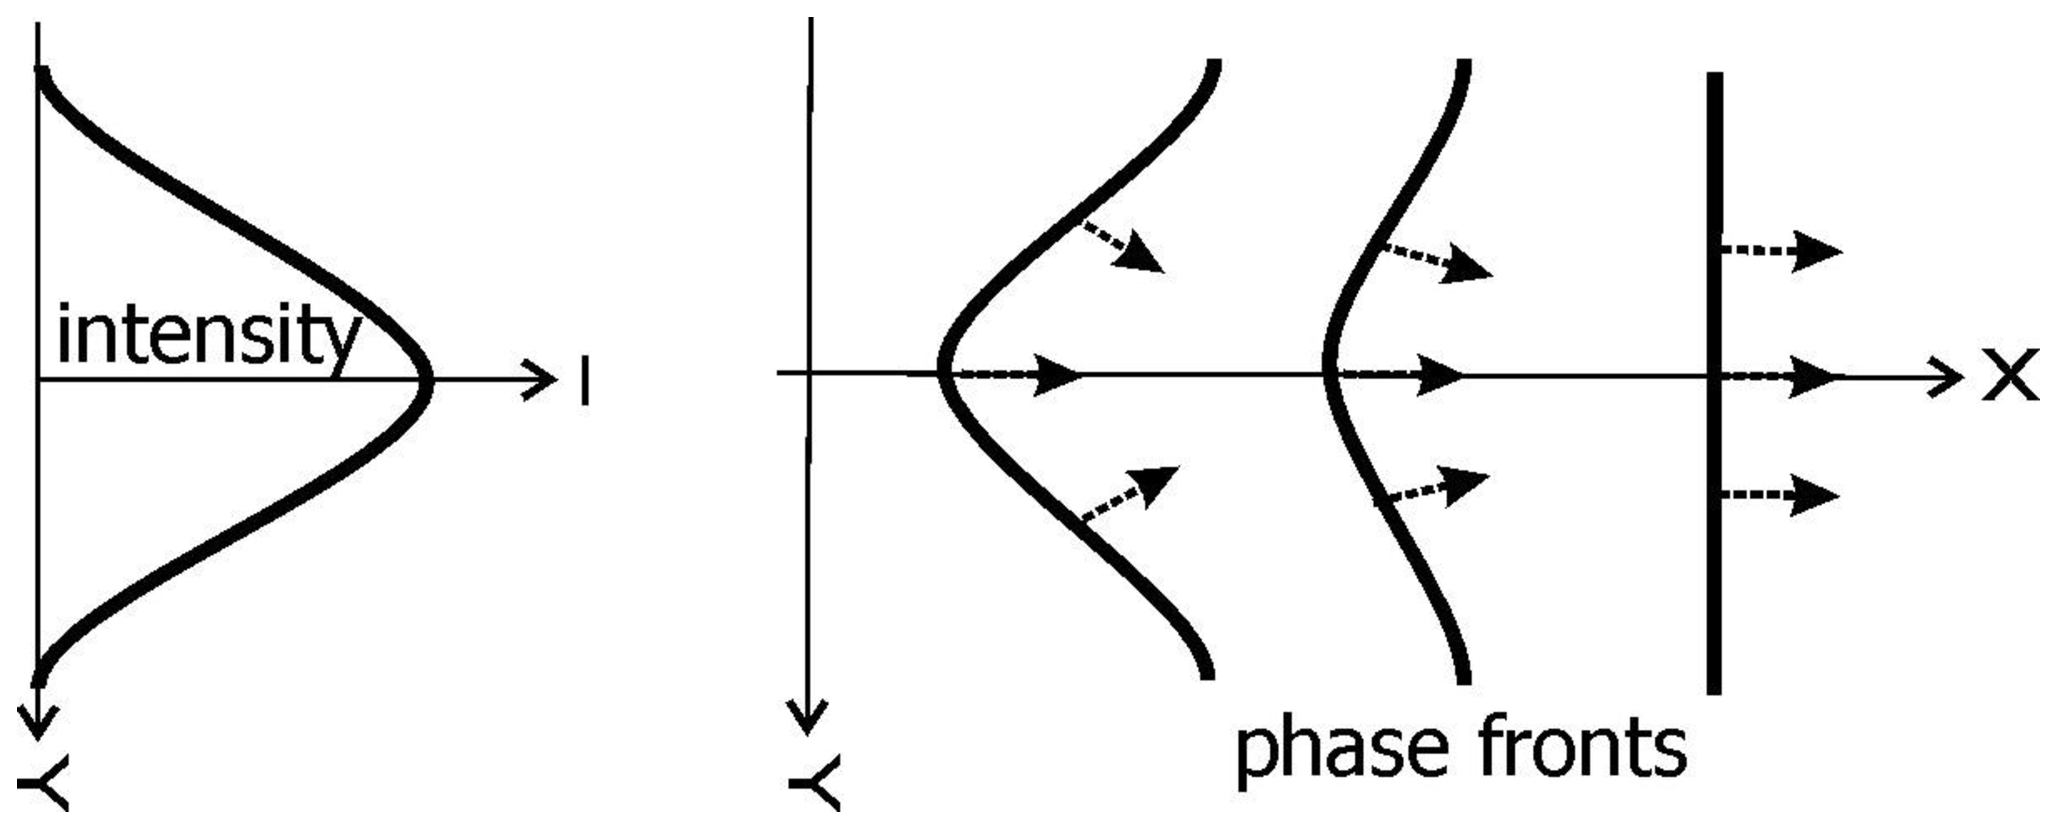
\includegraphics[width=\MyFactor\textwidth]{Img/selffocussing.eps}
  \caption{激光自聚焦示意图}
  \label{fig:selffousing}
\end{figure}

\begin{figure}[!htbp]
  \centering
  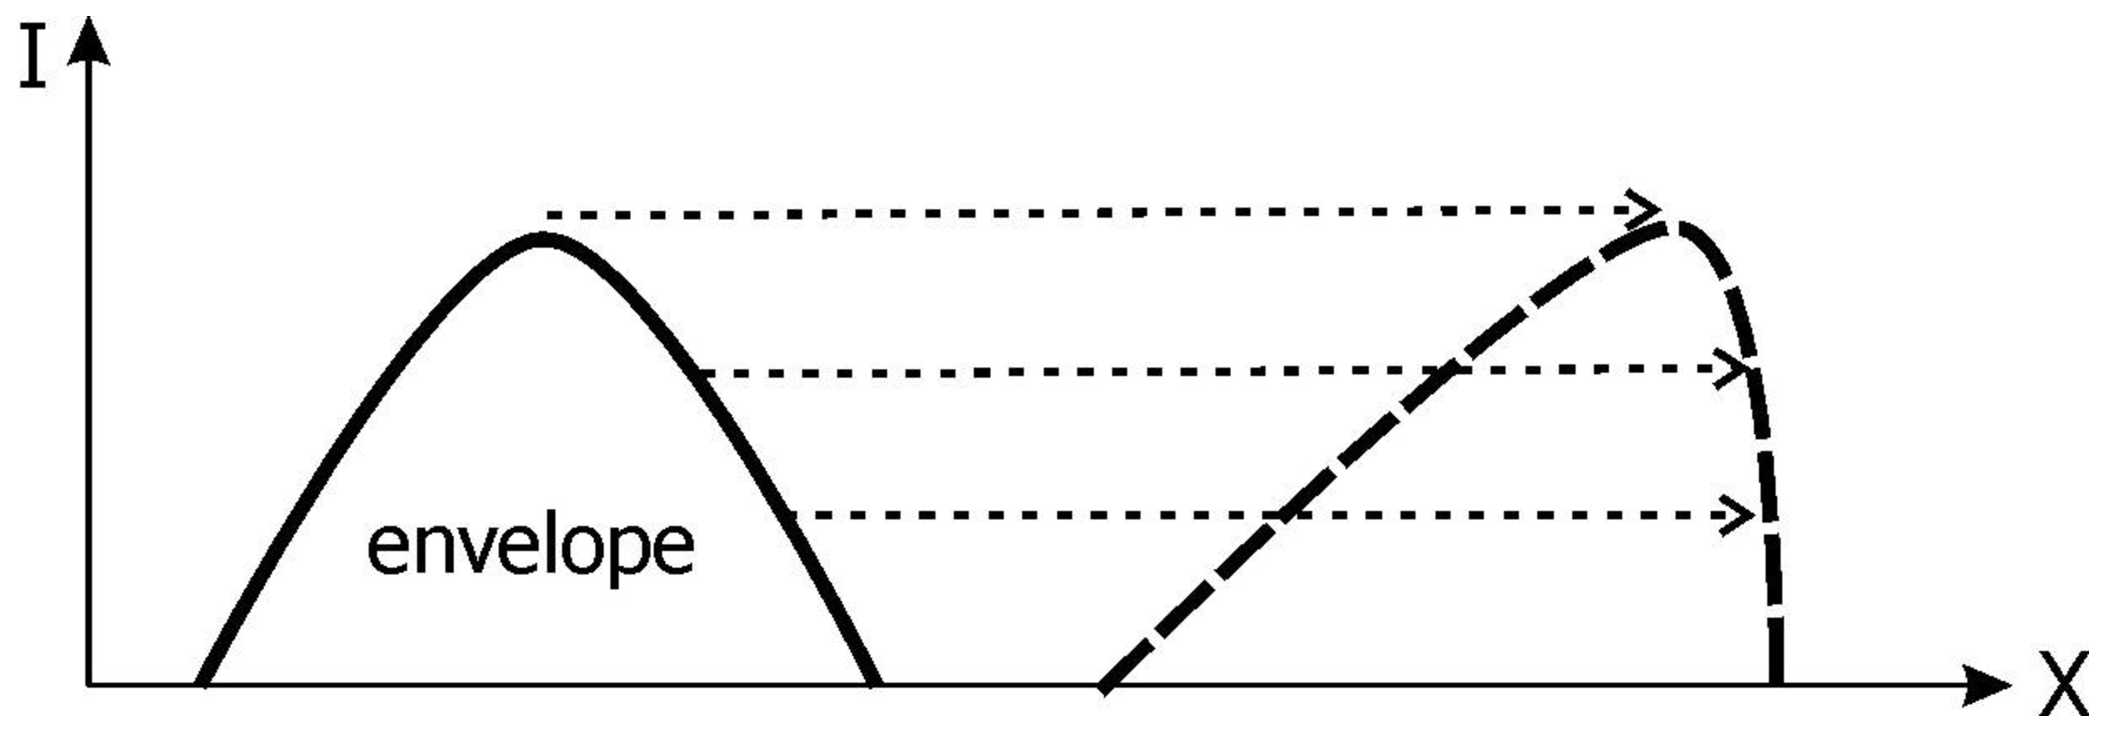
\includegraphics[width=\MyFactor\textwidth]{Img/prof-steepening.eps}
  \caption{激光自相位调制}
  \label{fig:phaseModulate}
\end{figure}

相对论激光脉冲在临界密度等离子体中,由于非线性现象的存在,其能量转换效率得到了很大的提高。正是因此,这一领域得到广泛的关注。早在1996年,A. Pukhov等就利用三维仿真程序VLPL研究了激光的自聚焦\cite{pukhov1996relativistic}进行了研究,观察到了相对论激光在临界密度等离子体中强烈的自聚焦,并对于聚焦条件以及现象进行了讨论。2011年王鸿勇人提出了相对论自聚焦透镜的模型\cite{wang2011laser},得到了最优的聚焦条件,并提出了利用透镜进行激光脉冲整形的观点。自聚焦透镜,是相对论强度激光在临界密度等离子体中传播中,当激光光强与等离子体密度匹配时,由自聚焦与自调制作用,使得激光在横向上焦斑变小纵向上脉冲尺寸压缩。经过透镜整形的激光脉冲,光强得到一个数量级的提高,同时激光的对比度明显地提高。
且在相对论激光脉冲在等离子体中传播的过程中,伴随着自聚焦,激光波前位置处的电子被激光有质动力排开,最终形成横向尺寸与激光焦斑大小离子背景的通道结构。通道中电子密度中间低两侧较高,形成了的静电势,而通道壁的电子由于回流效应产生轴向磁场。
在轴向磁场以及静电场的共同作用下,通道中的电子做betatron震荡,其频率由电磁场决定。同时,电子还受到激光场的驱动作用,当betatron震荡频率与激光频率匹配时,共振现象发生,使得电子对于激光产生强烈的能量吸收,这种现象被称为DLA(Direct Laser Acceleration)\cite{pukhov1998relativistic,pukhov1999particle}。其过程可解释为,共振电子的横向动量由于共振效应得到了很大的增益, 其横向震荡频率即激光频率$\omega_0$。在近稳态磁场的作用下,一部分的横向能量转化为纵向的能量, 横向以及纵向速度关系为$v_{\parallel} = 1- {v_{\perp}}^2$,由此得到纵向频率是$2 \omega_0$。DLA电子受到近稳态电磁场作用,在通道中紧聚焦,使得高能量密度电子束流沿激光传播方向运动,电子的温度的定标率,
\begin{equation}
\label{eqn:DLAtemperature}
T_e = 1.8(I_{cpa} {\lambda}^2/{13.7}GW)^{1/2}
\end{equation} 



1999年Gahn等\cite{gahn1999multi}的实验工作很好的验证了DLA理论。由于这种加速过程中,电子的运动类似自由电子激光中的wiggler,因此这种加速也被称为逆自由电子激光电子加速。其电子加热温度相对于传统的有质动力加速过程的电子温度, 有将近三倍以上的提高,而且由于通道中磁场的聚焦效果,因此电子束流的密度较高。
在此基础上,刘彬等提出自匹配共振电子加速理论,研究了DLA电子在通道中得到捕获过程,并给出了激光与等离子体的共振匹配条件。这种电子具有能量高且在时间以及空间上具有很强的谐振性,可用于高频率高品质的辐射的研究,是$\gamma$光源的重要途径。
\begin{figure}[!htbp]
  \centering
  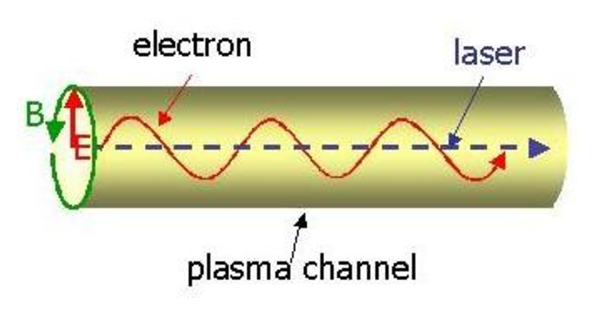
\includegraphics[width=\MyFactor\textwidth]{Img/IFEL.eps}
  \caption{逆自由电子激光示意图}
  \label{fig:IFEL}
\end{figure}
由于临界密度等离子中,激光能量耦合效率的显著提高,因此在离子加速研究中也有非常重要的应用。 Nakamura等人通过模拟发现,当激光在变化密度的临界密度等离子体中的传播时。激光可以穿透等离子体,并在其中稳定的传播,而当等离子体的密度发生突然变化的时候,在密度变化区域,一种磁场涡旋出现。这种磁涡旋结构的特点,纵向产生有效的加速电场,在横向产生对于离子的聚焦效应对于电子的散焦的效应。处于涡旋内部的质子被此结构捕获并得到能量增益,并且在纵向存在聚焦的效果。最终,可以实现准单能且强聚焦的离子束流。王鸿勇等人\cite{wang2011high}在2011年的理论工作提到,使用均匀临界密度的等离子体以及薄膜靶,可以实现3倍左右的能量提高,同时束流品质得到相应的提高。Sgattoni等人\cite{sgattoni2012laser}在2012通过二维以及三维的模拟细致地研究了激光在等离子体中的聚焦以及后续的加速的过程,最终也得到了质子能量明显增加的结论。在理论研究取得重要进步的同时,实验中,Mcknenna等人实现了预等离子体对于加速的增强效应。实验中使用中的强度烧蚀脉冲对于金属靶表面进行烧蚀的方法制备临界密度等离子体,其中与脉冲的持续时间可以控制,从而得到不同的预等离子体的分布。在进行了不同预脉冲尺寸的实验后,最终得到了最高能量38$MeV$的质子束流,相对于没有预脉冲的情况产生$25 \%$的能量提高。Glinec等\cite{glinec2008evolution}在2008年也完成的实验,使用不同强度以及脉冲长度的预脉冲控制预等离子体的分布,其结果表明,适度的烧蚀作用对于加速的作用是增强的,然而如果烧蚀脉冲过长,有可能起到负面的作用。然而此实验中很多的情况是可以优化的,而这一问题在后续将讨论。



\section{预等离子体增强离子加速}



以往的关于预等离子体对于加速的影响的研究工作中, 将临界密度等离子体对于离子加速的增强效应的原因归结为:1 激光脉冲在等离子体中的聚焦,使得激光的光强得到提高;2 高能电子的产生以及激光自聚焦的共同作用的结果。然而这种增强效果的根本原因是什么,如何在已有激光设备的基础上如何获得最优的质子加速效果,以及这种增强效果的潜能如何,这是本文的重点。


首先,我的问题在于如何制备预等离子体。传统的实验中,采用烧蚀脉冲作用于靶前表面产生预等离子体的方法,产生的等离子体在近临界密度区域呈现指数密度分布。可以通过控制烧蚀脉冲的参数控制指数密度分布的标度,具体可以参考上一章中的讨论。近年来,在临界密度等离子体的制备领域产生很重要的进步,Zoni等人2013年在实验上,利用间歇式脉冲激光实现了准均匀密度的泡沫等离子体的制备,其等离子体的密度以及厚度都可以得到有效的控制。2014年Passoni等人基于这种等离子体进行了质子加速的实验,使用非相对论强度的激光,最终的离子能量提高达到3倍之多。对于相对论强度激光,实验中增强效果不够明显。

对于激光离子加速,选取指数分布的等离子体以及均匀分布的等离子体,可作如下的分析。如果选取均匀密度等离子体,其初始密度符合DLA电子共振匹配条件,其激光与等离子体的能量耦合效率最高。然而自聚焦过程是动态的,聚焦过程中激光的强度得到增加,初始的匹配关系变得不再匹配,而激光的转化效率相应的变化。最终的能量耦合效率会低于预期的结果,因为激光脉冲与等离子体无法长时间匹配。 而对于变化密度的等离子体,随着激光自聚焦的强度增加,激光位置处等离子体的密度同时增加。如果可以保持匹配关系,激光的能量转换将处于最优情况,其必要条件是变化密度等离子体。为了简化模型,我们选取指数分布的等离子体密度,满足激光与等离子体的匹配问题。 针对这一观点,作相应的模拟工作:三组模拟中,激光以及固体靶参数保持一致,预等离子体的长度也相同,1号中为均匀密度分布,2号于3号为指数型密度分布,然而其标长不同。三组的电子能谱分布如图,以反映系统的能量转化效率。仿真结果表明,指数型分布的等离子体对于激光能量的吸收优于均匀密度分布的等离子体,同时指数分布的标长对于能量吸收有重要的影响。

基于上述的分析,本文中延续了实验中烧蚀脉冲作用于靶前表面产生预等离子体的方法,研究预脉冲产生的预等离子体对于加速的增强效应。强度$10^{12}\text{-}10^{14} W/cm^2$,脉冲时间$100ps$量级烧蚀脉冲与
$\mu m$量级的金属靶作用,烧蚀激光脉冲对于靶前表面离化加热,使得前表面的等离子体膨胀。通过调整烧蚀脉冲的强度以及持续时间,控制金属靶的烧蚀深度和预等离子体膨胀距离以及密度分布梯度,最终未烧蚀的靶和膨胀的等离子体形成了气体与固体薄膜靶的双层靶结构。气体靶的厚度在几十微米的量级,固体靶的厚度数微米,固体靶的作用是提供后表面形成鞘层加速场。 当主激光到来的时候,首先于气体作用,自聚焦的同时产生高能高密度的DLA共振电子。
激光能量有效地转化给电子,此电子束流MeV量级,在通道中得到有效的聚焦。此后电子穿透固体靶,靶中电子对于DLA电子产生散射作用,但是MeV量级电子在固体靶中的散射效应是可以忽略的。同时由于固体靶较薄(微米量级),DLA电子束流由于缺少聚焦作用的散射效应也不明显。 当电子传播至靶后,一部分电子回流至靶中,另一部分离开靶。此动态过程中,电子在靶后堆积并形成鞘层场加速离子,最终对于离子加速产生增强的作用。
DLA共振电子的温度$T_e=1.5(I_{cpa}{\lambda}^2/{13.7}GW)^{1/2}$\cite{pukhov1999particle},
相对于有质动力加热电子温度$T_e=0.5[(1+(I_{cpa}{\lambda}^2/{13.8}GW)/2)^{1/2}-1]$\cite{wilks1992absorption},有三倍的提高。当高密度高能DLA电子经过薄膜靶,在其后表面形成鞘层场,强度$E_{sheath}= (\frac{8 \pi}{e_N} n_e T_e)^{1/2}$ \cite{mora2003plasma}, $e_N \approx 2.71828$是欧拉常数。鞘层加速中的质子最高能量$E_{max} \propto T_e[In(2\tau)]^2$,其中 $\tau \propto \sqrt{n_e} \tau_{laser}$,$\tau_{laser}$是激光的脉冲持续时间。由加速电场以及最高能量的公式可知,电子的温度以及密度对于加速都有影响。同时提高电子的温度温度和密度,能实现最优的加速效果。首先需要把激光能量尽可能多的传递给电子,同时保证电子的密度。一方面,通过满足激光与等离子体之间的匹配关系,确保DLA共振电子加速转换尽可能多激光能量;另一方面,使得DLA电子处于通道的聚焦作用中,知道电子达到固体靶。具体的最优加速条件:
激光在即将达到固体靶的时候耗尽所有的能量,即DLA共振电子获得最大程度的能量增益的同时,确保激光脉冲产生的通道能够一直连接到金属靶,有助于电子保持聚焦的高密度状态。如果预等离子体的膨胀尺寸不够,激光脉冲有能量剩余,将直接作用于固体靶。其能量转化效率相对较低,电子得不到足够的能量而温度较低。相反,如果预等离子体的膨胀尺寸过长,激光会在预等离子体中可以完全吸收,然而此后通道随之消失,无法将高能量高密度DLA电子聚焦,电子传输到靶的过程中会产生一定的扩散导致密度降低。综合考虑共振电子的产生和传输过程,预等离子体的密度及尺寸决定了加速的增强效果。因此可以根据主激光与预等离子体的匹配关系控制预脉冲的参数,得到最优加速。为了简化模型,我们有如下的估计:


1共振电子产生于次临界密度等离子体,因为高密度区域由于密度匹配关系无法实现共振条件。而共振电子的数目
\begin{equation}
\label{eqn:DLAnumber}
\begin{cases}
N_e = \pi {{\sigma}_0}^2 {{\int}_{x_{front}}^{x_c}} density(x) dx  \\
density(x)=n_c exp(\frac{x-x_c}{c_s{\tau}_{abl}})
\end{cases}
\end{equation}
其中 $x_{front}$ 是预等离子体膨胀前沿, $x_c$ 临界密度面位置, 密度分布函数 $density(x)=n_c exp(\frac{x-x_c}{c_s{\tau}_{abl}})$ 是次临界密度等离子体的分布, $c_s \propto {I_{abl}^{1/3}}$ 等离子体声速,$I_{abl}$ 和 ${\tau}_{abl}$ 是烧蚀脉冲的强度以及脉冲持续时间。  
\begin{equation}
\label{eqn:DLAnumber1}
N_e = \pi {{\sigma}_0}^2 c_s {\tau}_{abl}[1-exp(\frac{x_{front}-x_c)}{{c_s{\tau}_{abl}}}]
\end{equation}
电子温度为 $T_e = 1.8(I_{cpa} {\lambda}^2/{13.7}GW)^{1/2}$,相应的共振电子能量:
\begin{equation}
\label{eqn:DLAenergy}
\begin{cases}
E_{absorb} = N_e{{\int}_{0}^{E_{max}}} f(E) dE = \\ 
N_e {{\int}_{0}^{E_{max}}} exp(-\frac{E}{T_e}) dE =  \\
N_e T_e (1-exp(-\frac{E_{max}}{T_e})) \approx N_e T_e
\end{cases}
\end{equation}
其中$f(E) = exp(-\frac{E}{T_e})$ 是能量分布函数。

2激光能量中一部分转化给通道中的共振电子,其转化比例为$\alpha_{absorb}$, 于是共振电子能量$E_{absorb} =\alpha_{absorb} E_{laser} $。激光脉冲能量
\begin{equation}
\label{eqn:laserEnergy}
E_{laser}=I_{cpa}{{\int}_{0}^{{\sigma}_0}} 2\pi r f_{rad}(r) dr {{\int}_{0}^{t_{max}}} f_{long}(t) dt
\end{equation}
其中$f_{rad}(r)$ 和 $f_{long}(t)$是激光的横向分布已经纵向包络, $I_{cpa}$ 和 $t_{max}$ 是激光的峰值光强以及脉冲持续时间。为了简化分析,我们取$f_{rad}(r)$和$f_{long}(t)$ 等于1,且$t_{max}=\tau_{cpa}$, $E_{laser}= \pi {{\sigma}_0}^2 \tau_{cpa} I_{cpa}$。对于其他的分布,结果有一个系数的差别。
\begin{equation}
\label{eqn:laserEnergy1}
E_{laser}= \pi {{\sigma}_0}^2 \tau_{cpa} I_{cpa}
\end{equation}


3激光与共振电子的能量转化存在极限值,$\alpha$在最优转化时达到极限值。
在以上假设的基础上,代换$E_{absorb}={\alpha}_{absorb} \times E_{laser}$,并归一化 $(I_{cpa} {\lambda}^2/{13.7}GW)^{1/2}$ 为 $a_{cpa}$, $(I_{abl} {\lambda}^2/{13.7}GW)^{1/2}$ 为 $a_{abl}$,且$c_s \propto {I_{abl}^{1/3}}$:

\begin{equation}
\label{eqn:OptimalCondition}
1.8 {a_{abl}}^{2/3} {\tau}_{abl}[1-exp((x_{front}-x_c)/{c_s{\tau}_{abl}})]  \propto {\alpha}_{absorb} a_{cpa} \tau_{cpa}
\end{equation}

对于百皮秒烧蚀脉冲,$(1-exp((x_{front}-x_c)/{c_s{\tau}_{abl}})) \approx 1 $,其中 $x_{front}-x_c= -{c_s {\tau}_{abl}}[2ln(\omega_{pi} {\tau}_{abl}) + ln2 -3]$ \cite{mora2003plasma},  $\omega_{pi}$ 是等离子体初始密度。在最优情况下,${\alpha}_{absorb}$是常数,此时预脉冲与主脉冲之间的匹配关系:
\begin{equation*}
\label{eqn:MatchEquation}
{a_{abl}}^{2/3} {\tau}_{abl} \propto a_{cpa} \tau_{cpa}
\end{equation*}

对于这一关系,我们做简单讨论。当$a_{cpa}$和$a_{abl}$固定是,简化为
\begin{equation*}
\label{eqn:MatchEquation1}
{\tau}_{abl} \propto \tau_{cpa} 
\end{equation*}
 直观的结论,长脉冲激光需要长预脉冲满足匹配关系,直观上增加激光能量就需要更多的预等离子体吸收这些能量。如果主激光的强度以及脉冲持续时间固定,则只有特定的预脉冲满足最优条件。实验上我们可以通过控制预脉冲的持续时间,满足最优加速条件。我们做了PIC模拟工作,检验上述模型。








在此理论分析基础上我们做了模拟仿真的研究,二维PIC粒子仿真,使用KLAP代码,参数依据北京大学强激光实验室条件,金属靶材质是密度为2.7$g/cm^3$铝靶,厚度为$\mu m$量级。激光参数包括有:预脉冲以及主脉冲。预脉冲的强度: $10^12W/cm^2$,且预脉冲的时间尺度为1ns之内。主激光脉冲在预脉冲之后,脉冲能量为5J,激光的脉冲持续时间为$30fs$,聚焦后的焦斑半径为5$\mu m$,相应强度$10^20W/cm^2$。靶结构为双层靶,10$\mu  m$量级的预等离子体与$\mu m$厚度的金属靶,其密度分布以及温度电离态等,由MULTI计算的结果导入。 PIC模拟中的参数如下:仿真区域$80 \times 40 \mu m^2$,格点数目$6400 \times 3200$, 其分辨率为$\lambda / 80$。仿真时间为200T, $T=3.3fs$为激光周期。通过改变预脉冲的持续时间,得到不同的密度分布,得出了三组仿真结果。



对于仿真的结果我们的分析如下:
首先分析出射质子能量最高组。激光在预等离子体中传播并将能量传递给共振电子的过程。如图所示(\ref{fig:laserEvolution}),在其中\ref{fig:laserEvolution}(a) 是激光聚焦的过程,$t=50T$的时候激光开始进入预等离子体,并在其中传播。之后$t=80$脉冲进入强聚焦的过程,激光的强度的增加剧烈,并且伴随着不稳定性的出现。$t=100T$激光波前达到金属靶的位置,其能量基本耗散。整个过程中,激光的能量很少有反射的成分,伴随着聚焦过程的增强,共振电子产生。在\ref{fig:laserEvolution}(b),电子的能量密度分布。 其中心位置处的电子呈现出明显的周期性结果,且其周期为激光的周期,而不是由于所谓的有质动力加速所产生的二倍于激光频率的结构。与此同时,紧聚焦的电子束流达到靶后,形成鞘层场,促进加速作用。在\ref{fig:laserEvolution}(c)显示了,激光脉冲耗散完之后离子通道的分布,其连接于靶前表面处,有效的保证了共振电子的束流品质。


\begin{figure}[!htbp]
  \centering
  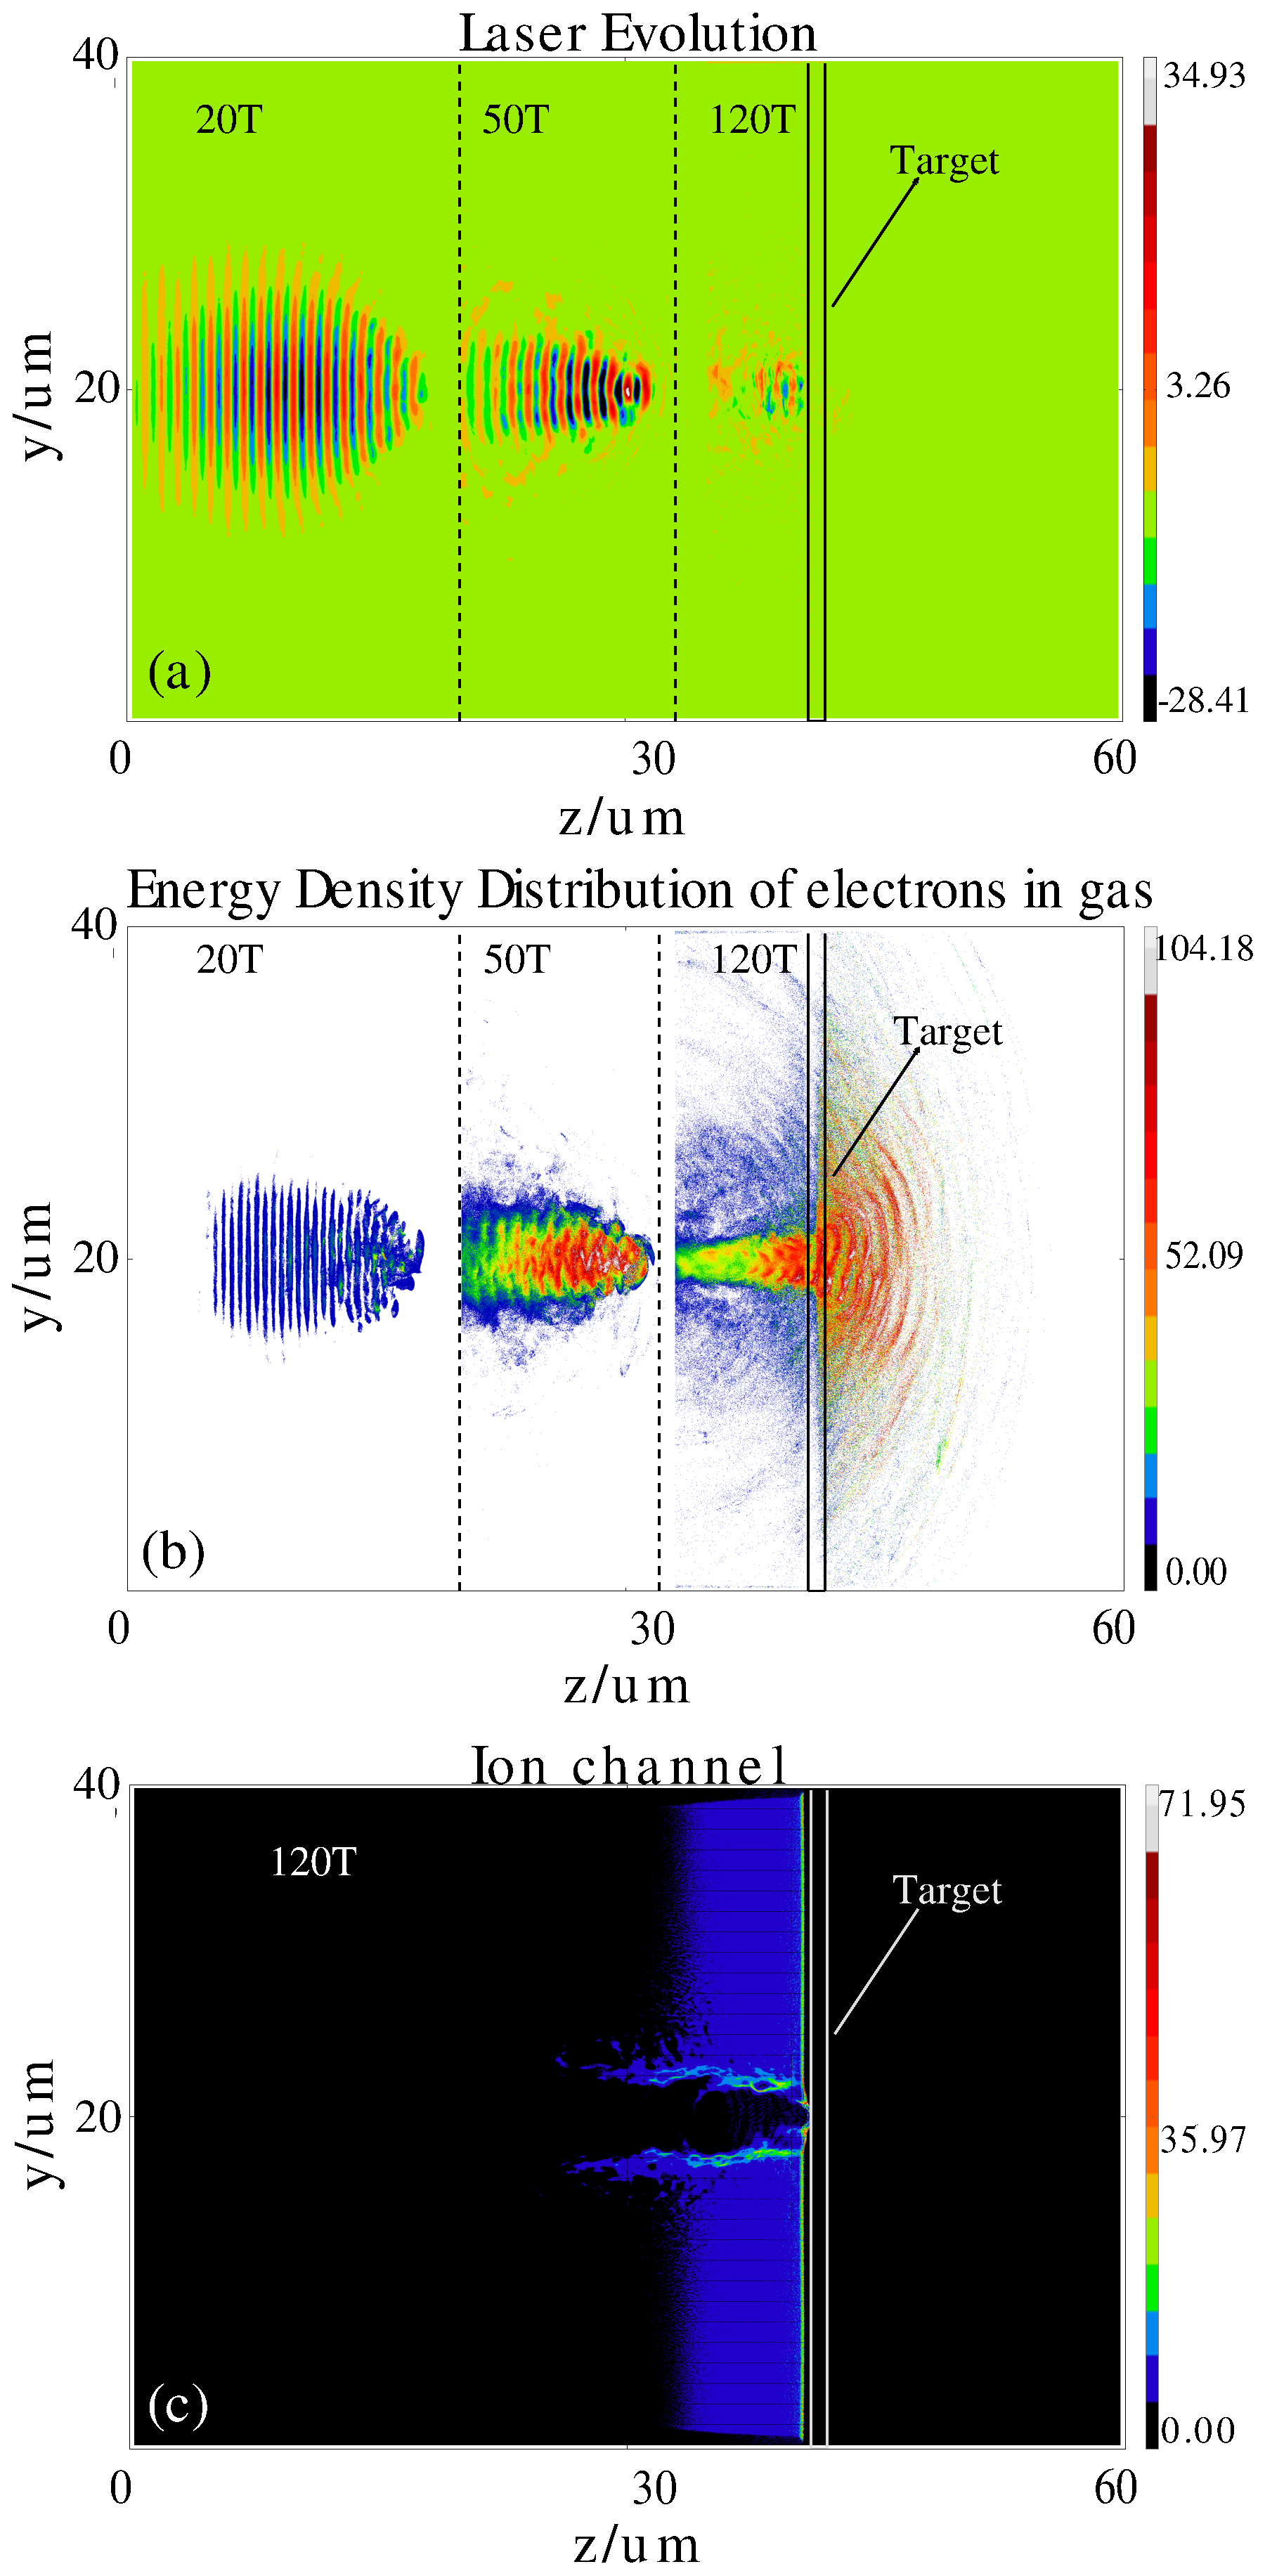
\includegraphics[width=\MyFactor\textwidth]{Img/laserEvolution.eps}
  \caption{激光聚焦及共振电子产生和传输}
  \label{fig:laserEvolution}
\end{figure}


另外两组能量较低的仿真结果在 \ref{fig:laserEvolution1} 中,其中一组,烧蚀脉冲的持续时间为100ps,称为‘短脉冲’,另一组的烧蚀脉冲持续时间为280ps,称为‘长脉冲’。不同的脉冲长度,对应的结果就是预等离子体密度分布的变化,其中‘短脉冲’对应的膨胀距离较小,而且等离子体的密度中梯度较大。而‘长脉冲’对应的等离子体的膨胀距离较大,而且密度梯度较小。同样做了激光脉冲聚焦在\ref{fig:laserEvolution1}(a)中, 左侧‘短脉冲’组中,激光在没有达到最优聚焦的时候已经被反射了,而右侧的激光脉冲在没有达到固体靶的时候已经完全的耗散,很显然,激光在‘长脉冲’组里的吸收更充分。对应于共振电子的产生的情况在\ref{fig:laserEvolution1}(b),其中‘短脉冲’中电子的能量密度较低原因在于激光能量未能完全的转化,右侧‘长脉冲’电子能量密度在 激光聚焦区域相对较高高。但是, 在‘长脉冲’中,由于激光在耗散之后,通道也就随之消失,没有相应的通道提供聚焦磁场,因此电子很快就散开。\ref{fig:laserEvolution1}(c)中给出了通道的形成,‘长脉冲’中,激光脉冲无法完全穿透预等离子体,从而无法实现通道连接到固体靶。 为了更好地理解等离子体中的电子的加热的情况,我们将电子的加热分区域进行了统计,包括:预等离子体中的电子以及固体靶中的电子。ref{fig:laserAbsorption}(b)为预等离子体中的电子加热的情况,其中红,黑,蓝分别代表着‘最优’,‘短脉冲’,‘长脉冲’的等离子体分布。‘最优’和‘长脉冲’的预等离子体中的电子加热情况类似,可见都已经达到了共振电子加热的极限的情况,而‘短脉冲’中的电子加热由于激光的吸收不完全,能量较低。在ref{fig:laserAbsorption}(c),统计了固体靶中的电子的能谱,‘最优’,‘长脉冲’情况中由于激光在达到靶的时候已经基本耗散,所有没有太多的能量沉积在固体靶子中,而对于‘较短’,电子的加热很明显,由于激光脉冲在固体靶表面有很强烈的反射,因此加热存在。考虑电子的平均温度以及数目,‘长脉冲’,‘最优’相对于‘较短’有着明显的优势,但是由于‘长脉冲’情况下,通道随于激光耗尽而消失,因此无法进一步进行共振电子的聚焦,造成了ref{fig:laserEvolution1}(d)所示的束流散开的情况,对于最终的加速有一定的影响。


\begin{figure}[!htbp]
  \centering
  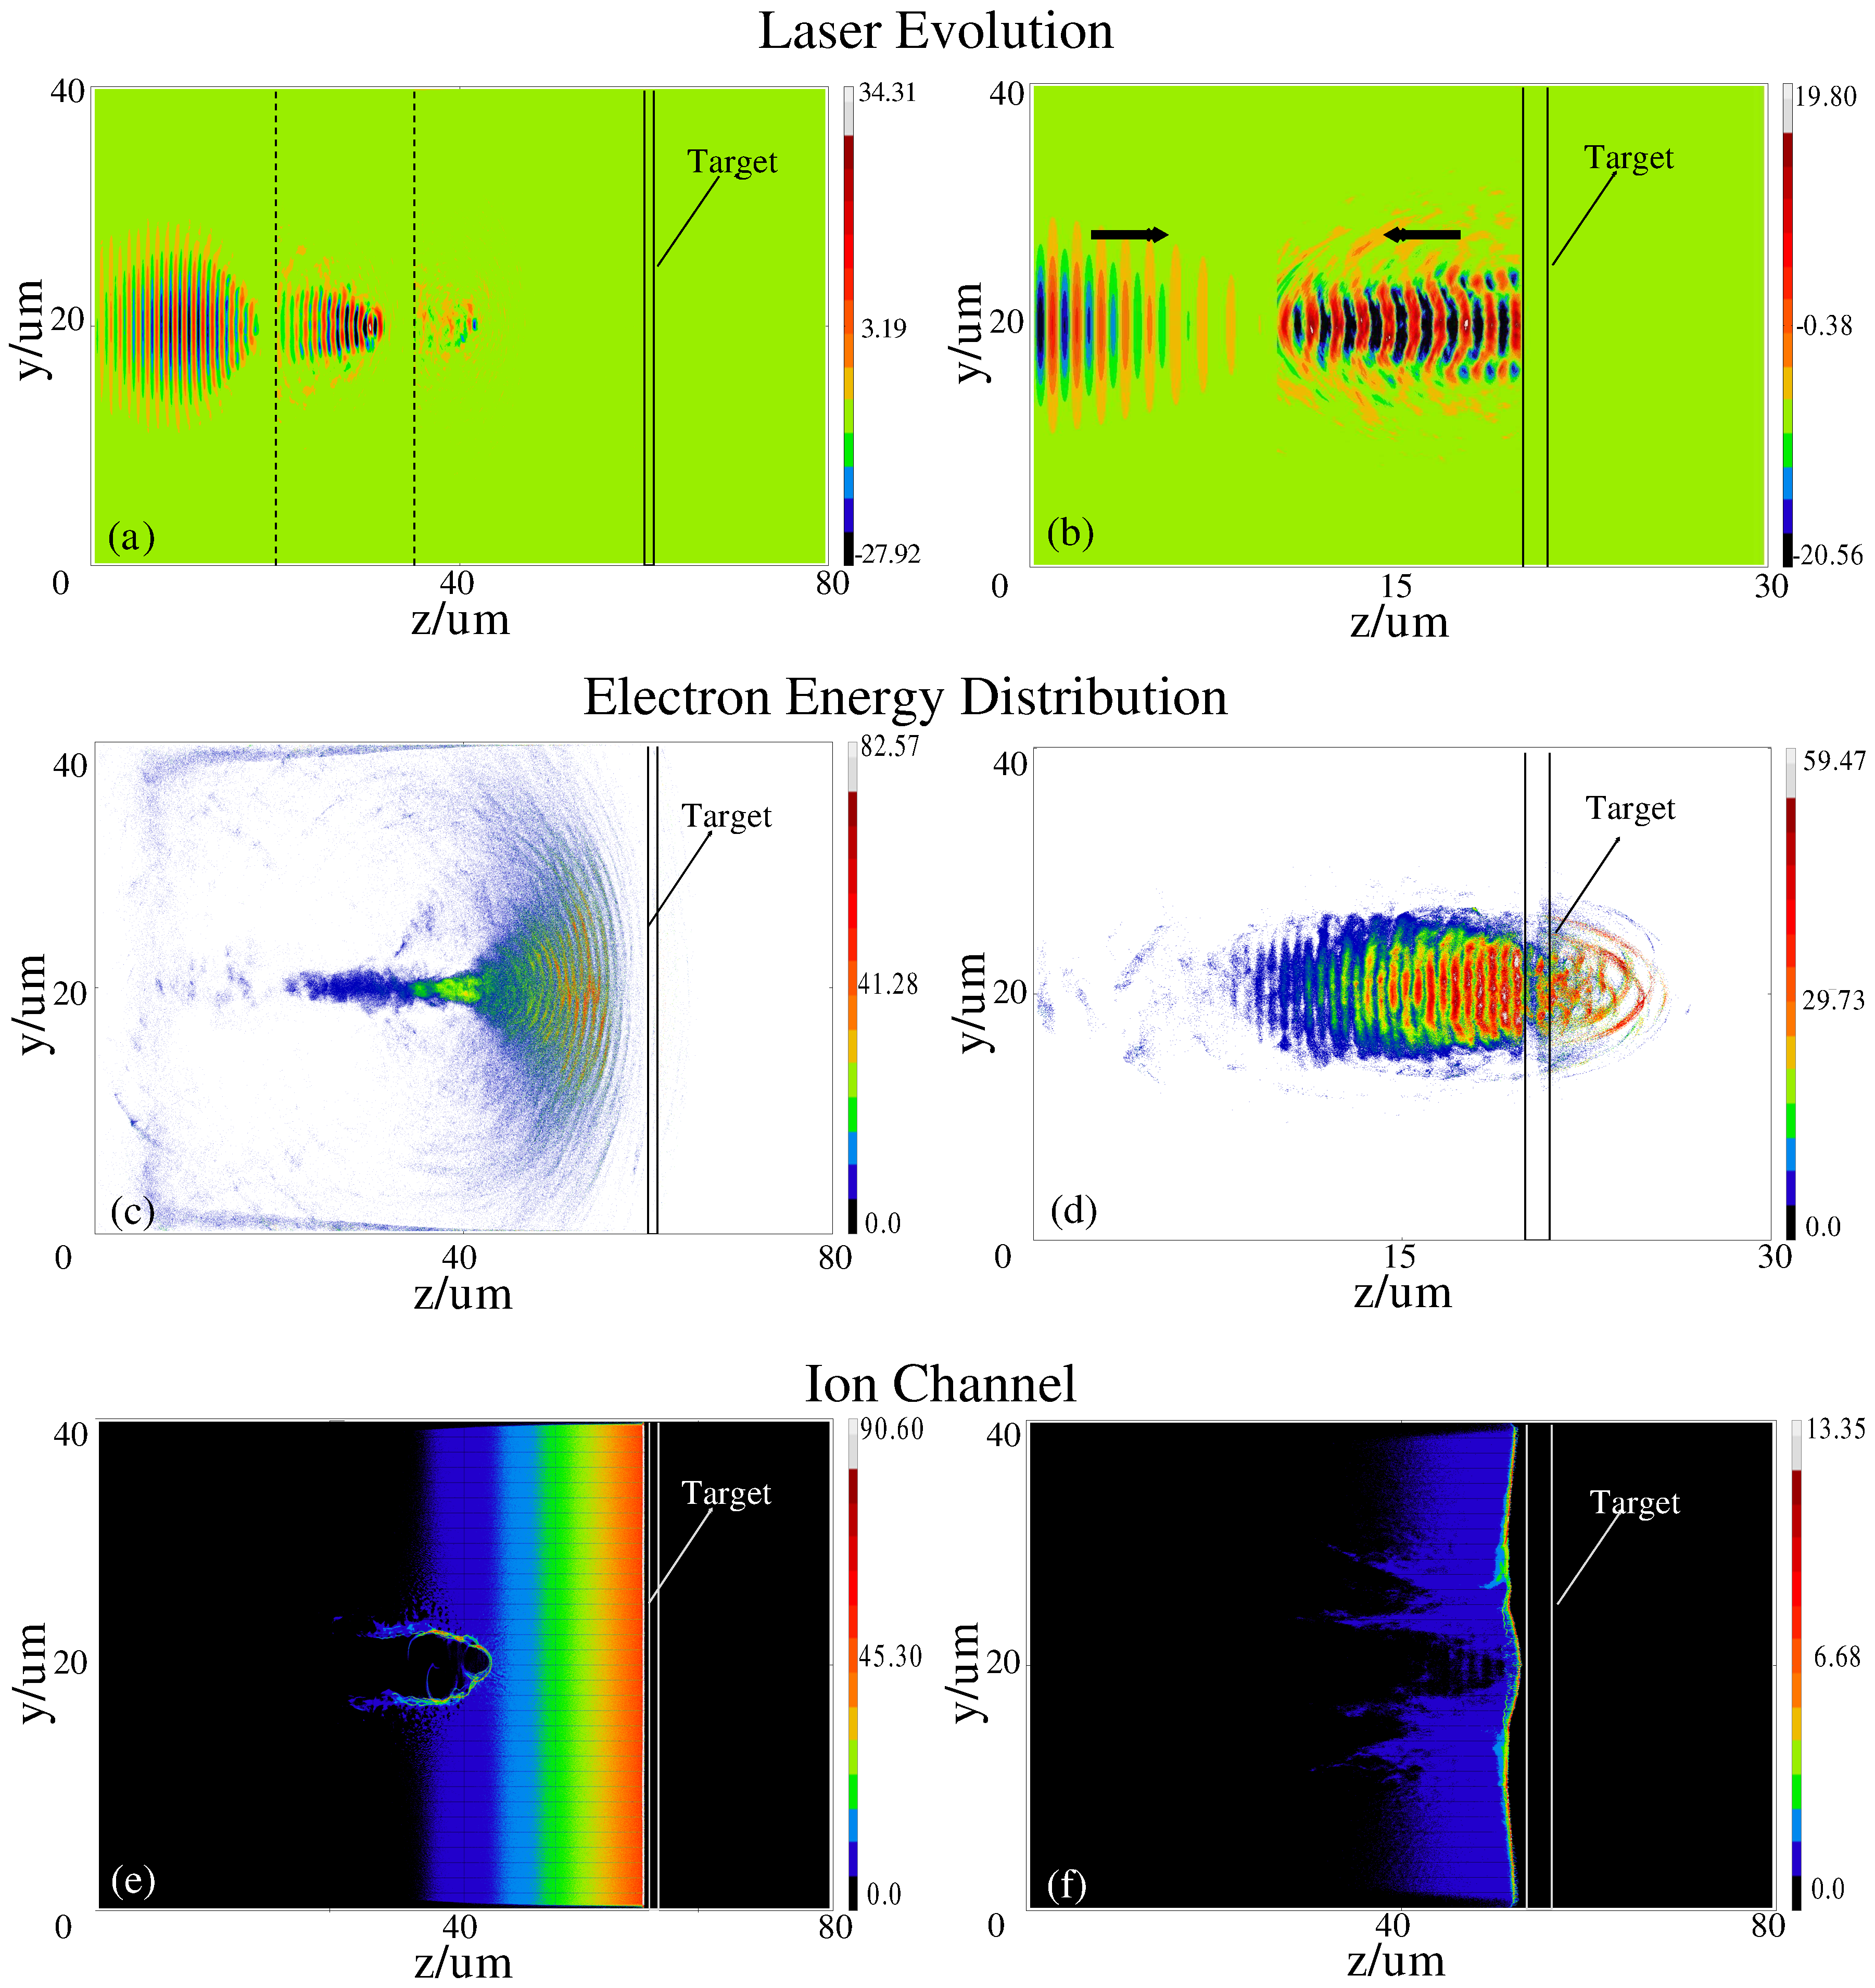
\includegraphics[width=\MyFactor\textwidth]{Img/laserEvolution1.eps}
  \caption{参照组中激光聚焦及共振电子产生和传输}
  \label{fig:laserEvolution1}
\end{figure}


对于以上三种情况,我们考虑了激光能量的吸收并得到了质子能谱,并使用没有预等离子体膨胀的情况进行参照,其结果在\ref{fig:laserAbsorption}(d)。能谱的统计采用了加速过程结束之后质子能量的统计,红色曲线代表‘最优’情况,其能量可以达到$90MeV$,蓝色的‘长脉冲’情况和黑色的‘短脉冲’情况相对较低,分别为$47MeV$,$65MeV$。但是对比绿色的‘无烧蚀’情况,质子能量都有显著提高。同时我们对最优情况,使用mora的自由膨胀的模型进行验证,电子的温度由\ref{eqn:DLAtemperature},而且电子的密度可以从模拟中得到相应的值,加速的时间可估计为$1.3 \tau_{laser}$\cite{fuchs2006laser},带入\ref{eqn:ionMaxenergy}中,得到加速的能量应该在90MeV。


\begin{figure}[!htbp]
  \centering
  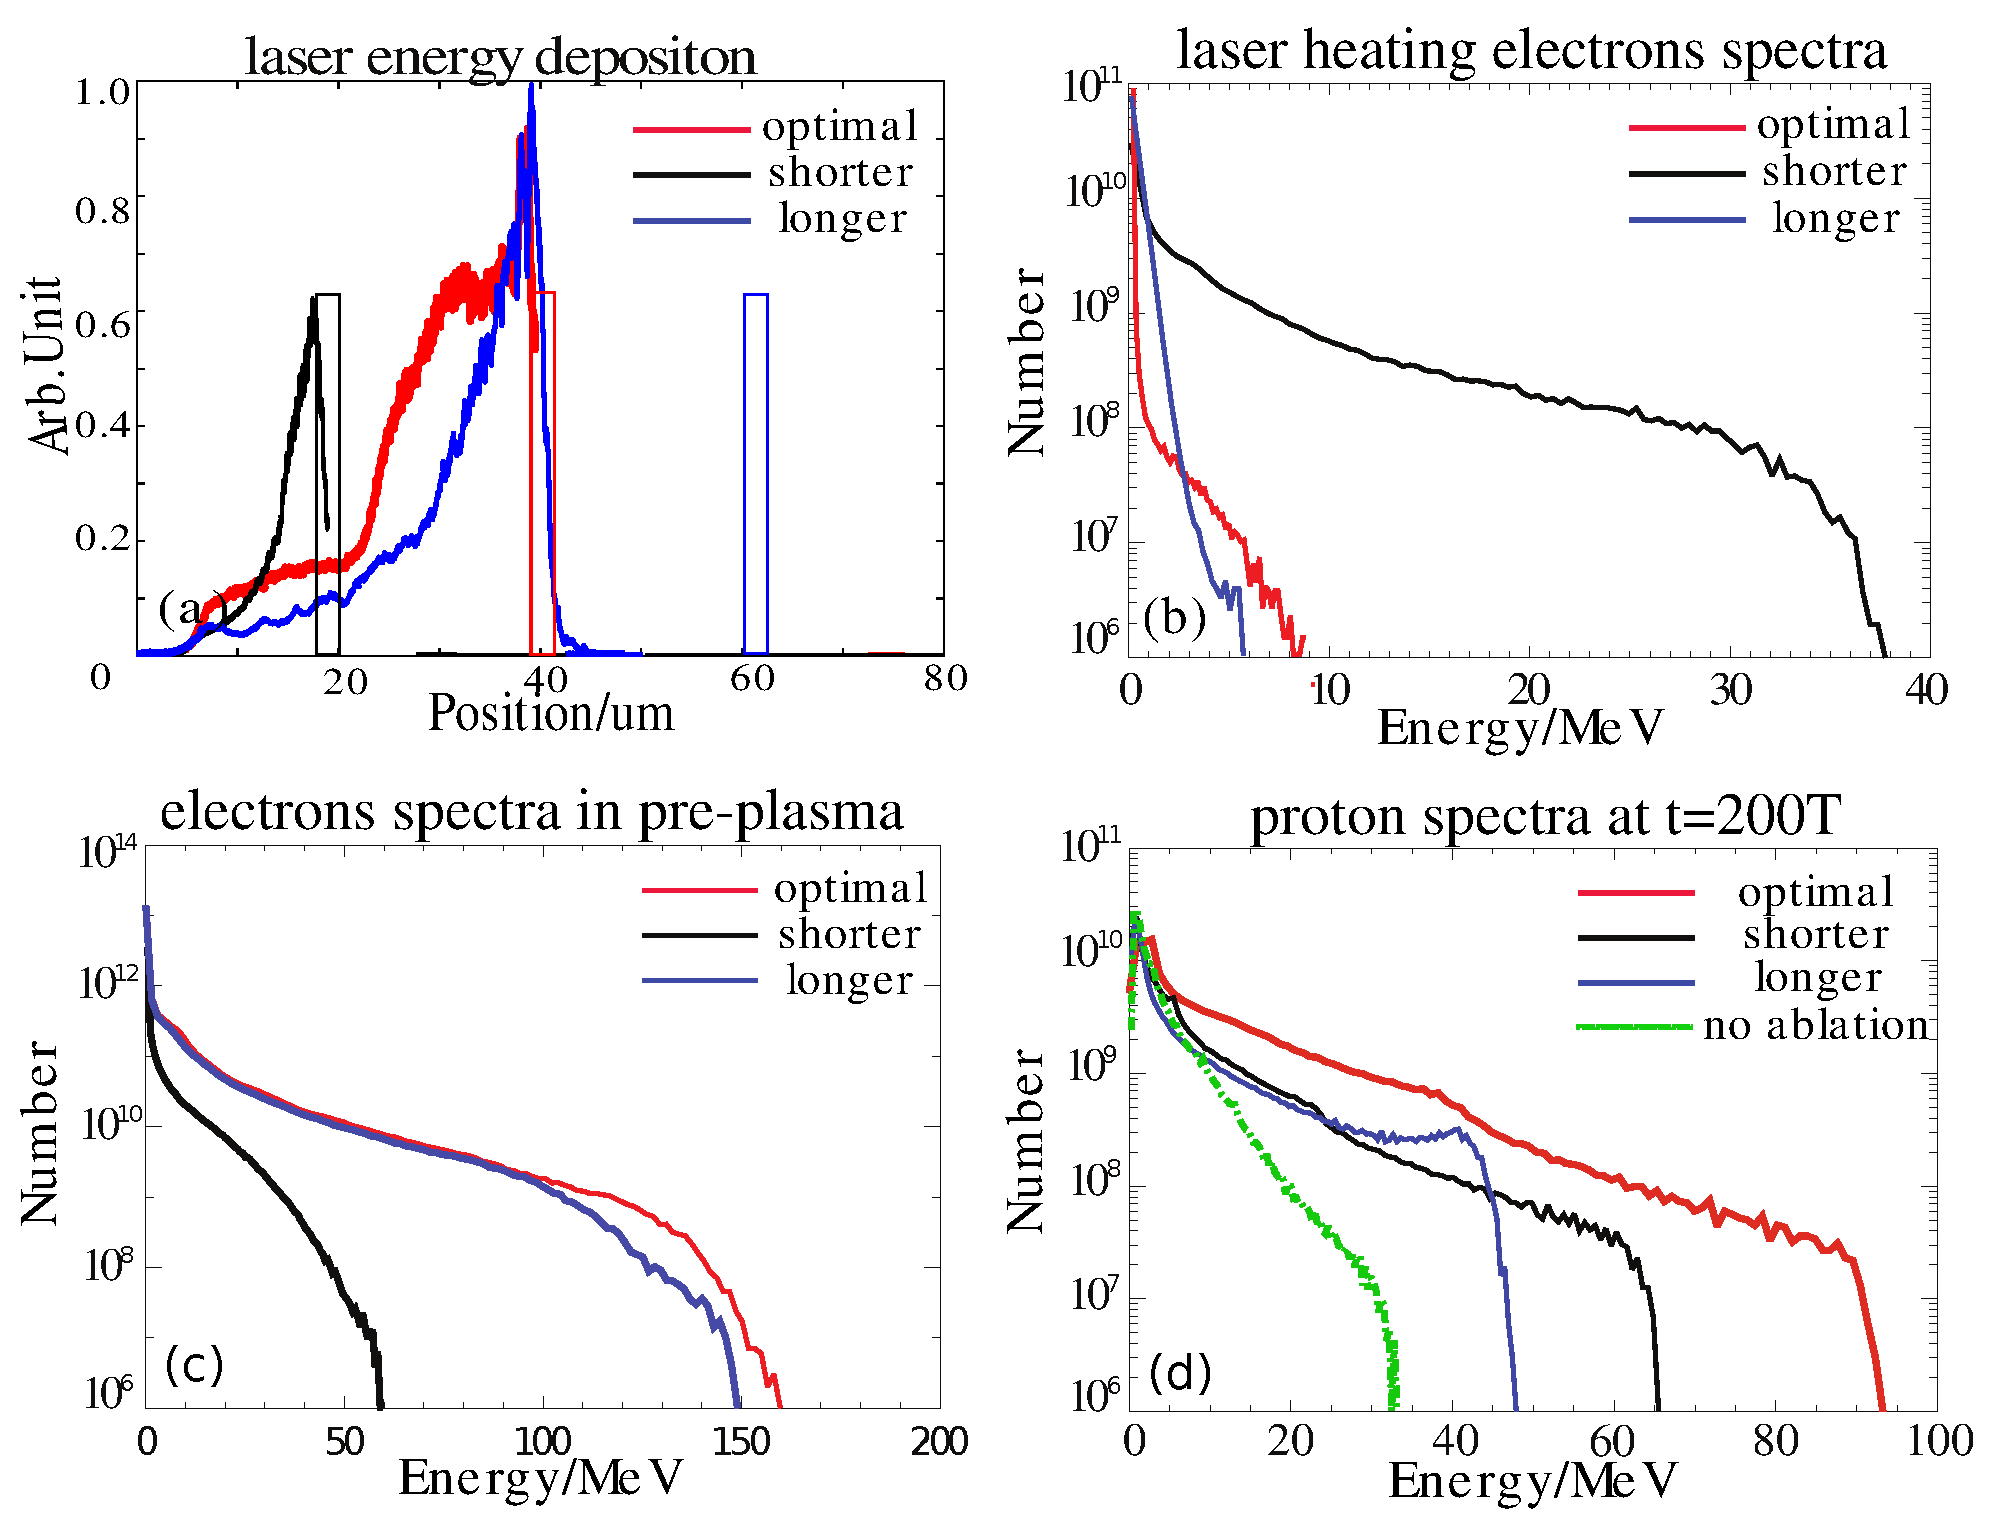
\includegraphics[width=\MyFactor\textwidth]{Img/laserAbsorption.eps}
  \caption{各组中激光能量的吸收}
  \label{fig:laserAbsorption}
\end{figure}



与此可见,由预脉冲产生的预等离子体对于质子加速可以起到增强的作用,而其增强效果存在最优的情况,对应于烧蚀脉冲与激光主脉冲之间的匹配关系。根据\ref{eqn:OptimalCondition},在固定预脉冲与主脉冲的强度的前提下,预脉冲的持续时间应该是和主脉冲的持续时间满足如下关系${\tau}_{abl} \propto  \tau_{cpa}$,呈现一定的正比关系。这就意味着,对于固定预脉冲以及烧蚀脉冲强度的情况,脉冲持续时间在匹配关系时,可以实现最优的增强效果。正如仿真中得到的结果, 脉冲持续时间过短或者过长的预脉冲都减弱了增强效果。在仿真中通过改变预脉冲以及主脉冲参数,得到预脉冲与主脉冲的匹配关系在\ref{fig:scanDuration}。散点是仿真结果,曲线是根据\ref{eqn:OptimalCondition}做出。二者在一定范围内符合,然而在脉冲宽度过大和过小的情况下,偏离了理论分析的结果。其原因在于,一些基本假设不再成立。例如:脉冲持续时间增长之后的能量吸收率不再是一个常量,而是和脉冲参数存在一定的关系;而在脉冲尺寸比较小的时候,由于激光与临界密度等离子体的作用时间不足,未能完全的进行能量转化,\ref{eqn:OptimalCondition}略微过估计了激光的吸收。


\begin{figure}[!htbp]
  \centering
  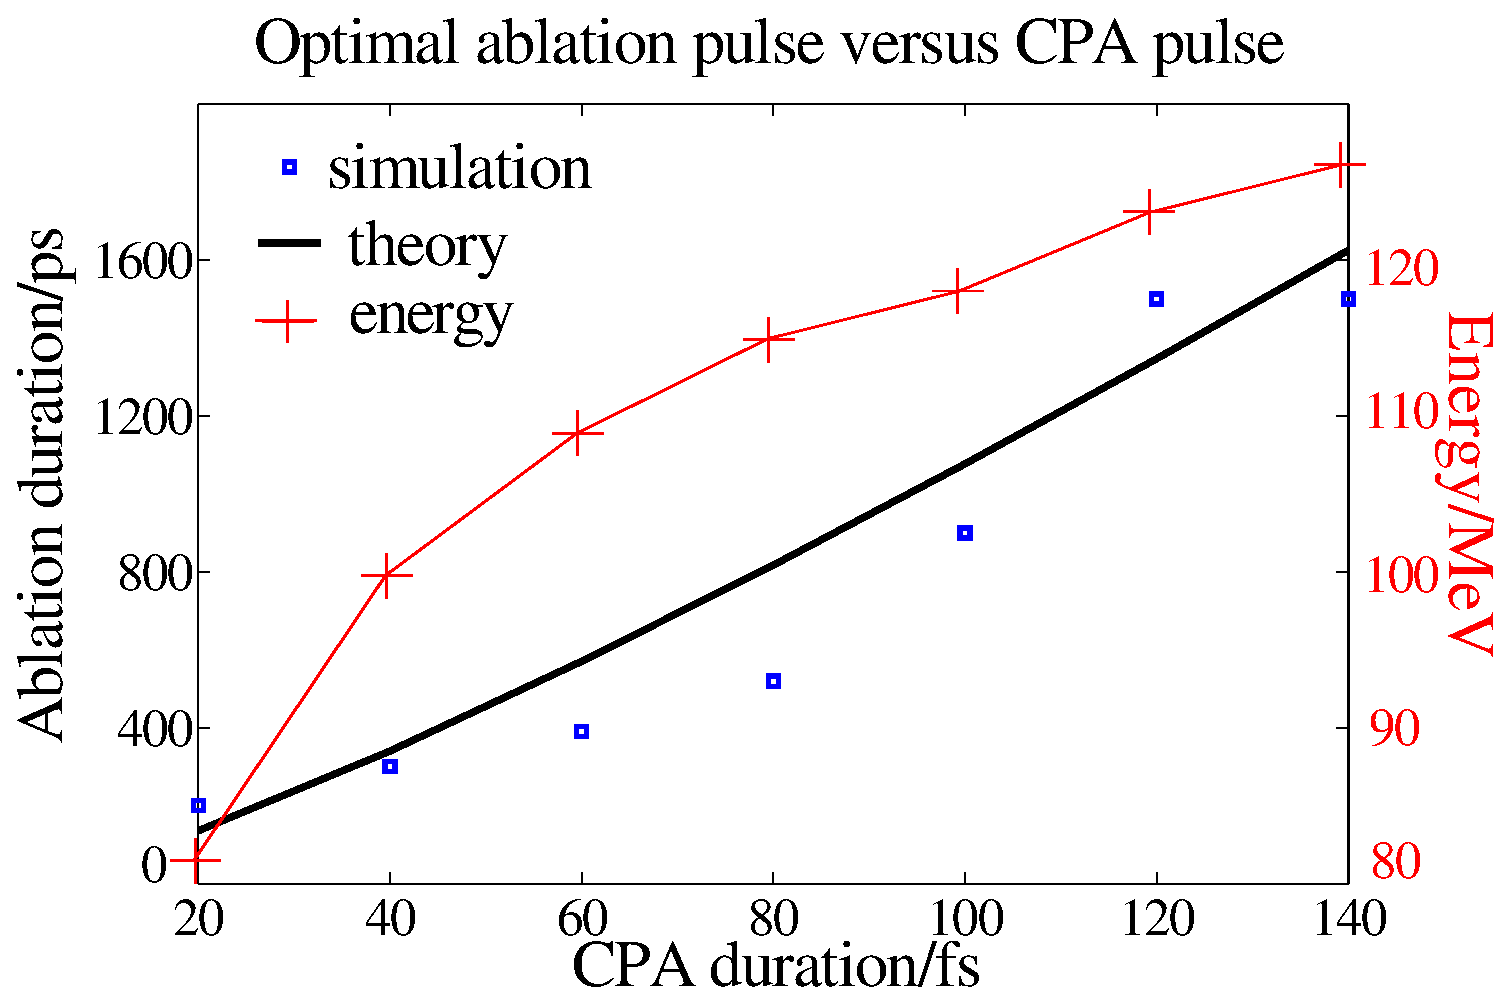
\includegraphics[width=\MyFactor\textwidth]{Img/scanDuration.eps}
  \caption{脉冲持续时间对于加速的影响}
  \label{fig:scanDuration}
\end{figure}



对于实验,我们有相应的实验的验证作为比较,在2008年,macknnea的实验就在一定程度上对于理论分析做出了相应的分析,因为在实验的参数如下,其强度与本文中的模拟的参数是近似的,烧蚀脉冲的持续时间以及主脉冲的持续时间相对较长,但是符合理论推导中的比例关系,因此间接证明了在较长的主脉冲的前提下,最优的加速过程对应于特定的一个激光的持续时间。同时实验中加速粒子的能量远远低于理论的预期的结果,很大原因是由于实验中使用的靶的厚度较大,25微米,这样的厚度下很难保证产生的高品质的共振电子部发生相应的发散,导致最终的及加速效果大打折扣。在实验中的脉冲持续时间是由于烧蚀脉冲的时间来决定的。烧蚀脉冲的时间用于控制激光等离子体的膨胀时间,而时间和膨胀的尺度存在直接的正比的关系,因此存在一定的关系决定最终的关于膨胀的尺度与激光脉冲的匹配关系,这一关系决定了相应的最优加速的过程是由于主脉冲激光和烧蚀脉冲的参数之间存在相应的匹配关系来决定的。一般来说,激光设备的主脉冲很难做出很大的调整,而相应的烧蚀脉冲由于其强度较低,控制的难度也相对较小,可以考虑通过控制烧蚀脉冲的强度以及脉冲持续时间来控制整个的加速的增强的过程。由于最优秀的加速过程往往存在唯一的对应的烧蚀脉冲,这对于实验中的控制是很有好处的,大大提高了相应的可控制的难度。




总的来说,使用预脉冲对于激光离子加速进行增强,是将传统意义上的‘有害’的预脉冲加以利用使其成为促进部分。  这一点对于实验有着一定的指导意义,通过调整烧蚀脉冲以及主脉冲的脉冲持续时间,改变加速离子的能量与束流的发散度,使得激光加速在一定程度上可控。从实验的可行性上,对于激光的控制在实验上更容易实现,对于给定的主脉冲激光,烧蚀激光可以使用激光预脉冲或者另一束独立的激光脉冲。控制其强度以及脉冲持续时间,使其满足最优增强效果,实现加速。




总结,预脉冲以及预等离子体在超强激光与等离子体作用的过程中是不可避免的,在离子加速的过程中,对于加速离子的能量可能起到正面或者反面的作用,直接与等离子体的密度分布有一定的关系,当等离子体的密度分布可以有助于产生共振电子的时候,由于激光的吸收得到有效的增强,进一步的加速的电子的效率得到显著的提升,而在另一方面,如果等离子体的密度的分布无法实现共振电子的条件,而且预脉冲由于强度比较的强,轻易的破坏掉了靶子的后表面结构,那么与等离子体起到的就是一种负面的作用因为无法通过破坏的加速面实现有效的加速电场的形成,在这种条件下的,加速就显得十分的没有意义了。 因此需要对于激光的与脉冲进行相应的控制,而这种控制的核心部分在于对于预脉冲的脉冲时间的控制。 因为时间的控制就决定了相应的预等离子体的分布。而且在给定的激光的强度以及激光的脉冲持续时间的基础上,有最优的预脉冲参数使得激光加速得到的离子的能量达到最高的值,这也是增强效果的最有意义的用途。在这样的基础上我们提出了使用烧蚀脉冲的方法对于传统的激光加速的方法进行相应的改进。烧蚀脉冲的参数考虑了实验室环境下常见的预脉冲的参数,并且对于不同预脉冲脉冲持续时间进行了深入的分析,得到了对于加速有最优效果的加速方案,因为在此基础上的加速,将最大化的实现激光到离子的能量转化。综合考虑实验的可行性,以及加速增强效果,这种方案可以使一种在现有的实验室环境下 的有效的方法,且其操作性强,需要控制的是激光的参数,而不是进行微结构的靶的制作,相应的技术层面的要求更合适目前的实验室的环境的需求。对比于没有烧蚀脉冲的情况,得到的加速的质子的能量提高了响应的3倍以上的量。相信这种技术可以在实验中取得相应的突破,使得激光离子加速的能量步入到百MeV的数量级。此方案的一个优势在于变废为宝,因为在实验中不需要引进 外界的参量,需要的是性能稳定的激光器设备以及分光技术,使得激光的脉冲可以被分成两部分一部分通过放大技术成为主脉冲,另一部分则可以完全用来当做烧蚀脉冲实现对于靶的烧蚀。在这样的设计中,很重要的一点就是主激光以及烧蚀激光之间的匹配关系,因为预脉冲的持续时间决定了相应的预等离子体的分布的情况。在预等离子体中的共振电子的产生是加速增强的直接的原因,没有主激光与预脉冲之间的匹配关系,就很难真的存在对于加速的最优的增强的效果。这是整个章节的核心的地方,也是这种方案的核心,是对于加速在一定程度上进行了相应的控制使得加速的离子的能力可以满足在一定的范围的分布,而且离子的束流的发散程度是和激光的参数相关的,实现了相应的关于控制的要求。



